\propriete[\exmplist{27,32 + 18,1 devient :\\ \opadd{27.32}{18.1}}{8768+12792 devient :\\ \opadd{8768}{12792}}{0,0001+11,2 devient :\\ \opadd{0.0001}{11.2}}]
{Poser un addition}
{On va ici poser l'addition 12,83 + 3, 41.\\    
\begin{minipage}{0.7\textwidth}    
On pose les deux nombres à additionner l'un en dessous de l'autre, en alignant les chiffres des unités. 
\end{minipage}
\hfill
\begin{minipage}{0.22\textwidth}
    \begin{figure}[H]
    \centering
        \resizebox{\textwidth}{!}{
            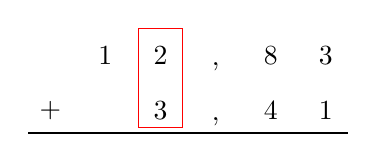
\begin{tikzpicture}[scale=0.7]
                \draw (0,0) node {1} ;
                \draw (1,0) node {2} ; 
                \draw (2,-0.2) node {,} ;
                \draw (3,0) node {8} ;
                \draw (4,0) node {3} ;
                \draw (1,-1) node {3} ; 
                \draw (2,-1.2) node {,} ;
                \draw (3,-1) node {4} ;
                \draw (4,-1) node {1} ;
                \draw (-1,-1) node {+} ;
                \draw (-1.4,-1.4) -- (4.4,-1.4) ;
                \draw [red] (0.6,0.5) rectangle (1.4,-1.3);
            \end{tikzpicture}
        }
    \end{figure}
\end{minipage}
\begin{minipage}{0.7\textwidth}    
    Si il y a des virgules, elles doivent ainsi être alignées. La virgule du résultat final sera aussi alignée. 
\end{minipage}
\hfill
\begin{minipage}{0.22\textwidth}
    \begin{figure}[H]
    \centering
        \resizebox{\textwidth}{!}{
            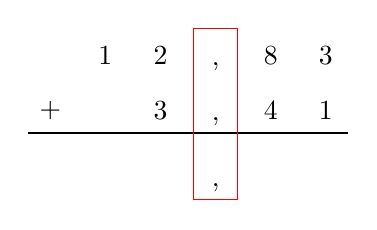
\begin{tikzpicture}[scale=0.7]
                \draw (0,0) node {1} ;
                \draw (1,0) node {2} ; 
                \draw (2,-0.2) node {,} ;
                \draw (3,0) node {8} ;
                \draw (4,0) node {3} ;
                \draw (1,-1) node {3} ; 
                \draw (2,-1.2) node {,} ;
                \draw (3,-1) node {4} ;
                \draw (4,-1) node {1} ;
                \draw (-1,-1) node {+} ;
                \draw (-1.4,-1.4) -- (4.4,-1.4) ;
                \draw (2,-2.4) node {,} ;
                \draw [red] (1.6,0.5) rectangle (2.4,-2.6);
            \end{tikzpicture}
        }
    \end{figure}
\end{minipage}
\begin{minipage}{0.7\textwidth}    
    Puis on additionne les chiffre colones par colones, de gauche à droite, en écrivant le résultat sous la colone. 
\end{minipage}
\hfill
\begin{minipage}{0.22\textwidth}
    \begin{figure}[H]
    \centering
        \resizebox{\textwidth}{!}{
            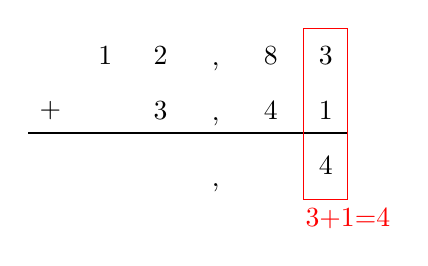
\begin{tikzpicture}[scale=0.7]
                \draw (0,0) node {1} ;
                \draw (1,0) node {2} ; 
                \draw (2,-0.2) node {,} ;
                \draw (3,0) node {8} ;
                \draw (4,0) node {3} ;
                \draw (1,-1) node {3} ; 
                \draw (2,-1.2) node {,} ;
                \draw (3,-1) node {4} ;
                \draw (4,-1) node {1} ;
                \draw (-1,-1) node {+} ;
                \draw (-1.4,-1.4) -- (4.4,-1.4) ;
                \draw (2,-2.4) node {,} ;
                \draw (4,-2) node {4} ;
                \draw [red] (3.6,0.5) rectangle (4.4,-2.6) node[below] {3+1=4};
            \end{tikzpicture}
        }
    \end{figure}
\end{minipage}
\begin{minipage}{0.7\textwidth}    
    Si le résultat est supérieur ou égal à 10, on écrit seulement le chiffre des unités sous la colone. Le chiffre des dizaine, lui, est rajouté à la colone suivante (celle de gauche). On appelle ceci une retenue.
\end{minipage}
\hfill
\begin{minipage}{0.22\textwidth}
    \begin{figure}[H]
    \centering
        \resizebox{\textwidth}{!}{
            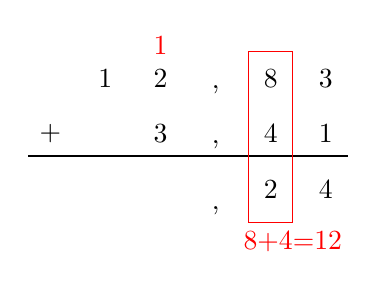
\begin{tikzpicture}[scale=0.7]
                \draw (0,0) node {1} ;
                \draw (1,0) node {2} ; 
                \draw (2,-0.2) node {,} ;
                \draw (3,0) node {8} ;
                \draw (4,0) node {3} ;
                \draw (1,-1) node {3} ; 
                \draw (2,-1.2) node {,} ;
                \draw (3,-1) node {4} ;
                \draw (4,-1) node {1} ;
                \draw (-1,-1) node {+} ;
                \draw (-1.4,-1.4) -- (4.4,-1.4) ;
                \draw (2,-2.4) node {,} ;
                \draw (4,-2) node {4} ;
                \draw (3,-2) node {2} ;
                \draw [red] (2.6,0.5) rectangle (3.4,-2.6) node[below] {8+4=12};
                \draw[red] (1,0.6) node {1} ;
            \end{tikzpicture}
        }
    \end{figure}
\end{minipage}
\begin{minipage}{0.7\textwidth}    
    Lors du calcul d'une colone avec une retenue, on additionne le chiffre retenu aux autres, on écrit le résultat en bas de la colone, et on continue.
\end{minipage}
\hfill
\begin{minipage}{0.22\textwidth}
    \begin{figure}[H]
    \centering
        \resizebox{\textwidth}{!}{
            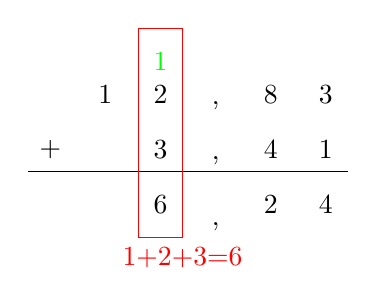
\begin{tikzpicture}[scale=0.7]
                \draw (0,0) node {1} ;
                \draw (1,0) node {2} ; 
                \draw (2,-0.2) node {,} ;
                \draw (3,0) node {8} ;
                \draw (4,0) node {3} ;
                \draw (1,-1) node {3} ; 
                \draw (2,-1.2) node {,} ;
                \draw (3,-1) node {4} ;
                \draw (4,-1) node {1} ;
                \draw (-1,-1) node {+} ;
                \draw (-1.4,-1.4) -- (4.4,-1.4) ;
                \draw (2,-2.4) node {,} ;
                \draw (4,-2) node {4} ;
                \draw (3,-2) node {2} ;
                \draw (1,-2) node {6} ;
                \draw [red] (0.6,1.2) rectangle (1.4,-2.6) node[below] {1+2+3=6};
                \draw[green] (1,0.6) node {1} ;
            \end{tikzpicture}
        }
    \end{figure}
\end{minipage}
\begin{minipage}{0.7\textwidth}    
    S'il n'y a qu'un seul chiffre dans une colone, on l'écrit directement en bas de celle-ci.
\end{minipage}
\hfill
\begin{minipage}{0.22\textwidth}
    \begin{figure}[H]
    \centering
        \resizebox{\textwidth}{!}{
            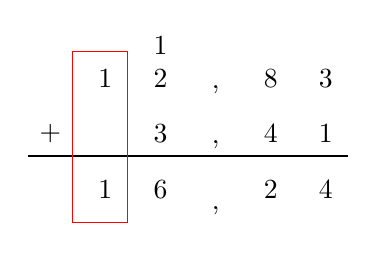
\begin{tikzpicture}[scale=0.7]
                \draw (0,0) node {1} ;
                \draw (1,0) node {2} ; 
                \draw (2,-0.2) node {,} ;
                \draw (3,0) node {8} ;
                \draw (4,0) node {3} ;
                \draw (1,-1) node {3} ; 
                \draw (2,-1.2) node {,} ;
                \draw (3,-1) node {4} ;
                \draw (4,-1) node {1} ;
                \draw (-1,-1) node {+} ;
                \draw (-1.4,-1.4) -- (4.4,-1.4) ;
                \draw (2,-2.4) node {,} ;
                \draw (4,-2) node {4} ;
                \draw (3,-2) node {2} ;
                \draw (1,-2) node {6} ;
                \draw (0,-2) node {1} ;
                \draw [red] (-0.6,0.5) rectangle (0.4,-2.6) ;
                \draw (1,0.6) node {1} ;
            \end{tikzpicture}
        }
    \end{figure}
\end{minipage}
\\\vspace{1em}\\
Après avoir fait la dernière colone, on lit le résultat sur la ligne du bas. Donc  12,83+3,41=16,24.
}
